\documentclass{sig-alternate-05-2015}
\usepackage[utf8]{inputenc}
\usepackage[italian]{babel}
\usepackage[T1]{fontenc}
\usepackage{graphicx}
\usepackage{graphics}
\usepackage{listings}  
\usepackage{array}
\newcolumntype{L}[1]{>{\raggedright\let\newline\\\arraybackslash\hspace{0pt}}m{#1}}
\newcolumntype{C}[1]{>{\centering\let\newline\\\arraybackslash\hspace{0pt}}m{#1}}
\newcolumntype{R}[1]{>{\raggedleft\let\newline\\\arraybackslash\hspace{0pt}}m{#1}}
\usepackage{multirow}
\usepackage[table]{xcolor}
\usepackage{float}
\usepackage{array}
\usepackage{ragged2e}
\newcolumntype{P}[1]{>{\RaggedRight\hspace{0pt}}p{#1}}

\usepackage{etoolbox}
\makeatletter
\patchcmd{\@makecaption}
{\scshape}
{}
{}
{}
\makeatother

\newcolumntype{"}{@{\hskip\tabcolsep\vrule width 1pt\hskip\tabcolsep}}

\lstdefinestyle{base}{
	language=C,
	emptylines=1,
	breaklines=true,
	basicstyle=\ttfamily\color{black},
	moredelim=**[is][\color{red}]{@}{@},
}

\newcommand{\squeezeup}{\vspace{-2.5mm}}
\newcommand\FIXME[1]{\textbf{FIXME: #1}}

\begin{document}

% Copyright
\setcopyright{acmcopyright}
%\setcopyright{acmlicensed}
%\setcopyright{rightsretained}
%\setcopyright{usgov}
%\setcopyright{usgovmixed}
%\setcopyright{cagov}
%\setcopyright{cagovmixed}


%% DOI
%\doi{10.475/123_4}

%% ISBN
%\isbn{123-4567-24-567/08/06}

%Conference
\conferenceinfo{MSR '17}{May 20--21, 2017, Buenos Aires, Argentina}

%\acmPrice{\$15.00}

%
% --- Author Metadata here ---
%\conferenceinfo{WOODSTOCK}{'97 El Paso, Texas USA}
%\CopyrightYear{2007} % Allows default copyright year (20XX) to be over-ridden - IF NEED BE.
%\crdata{0-12345-67-8/90/01}  % Allows default copyright data (0-89791-88-6/97/05) to be over-ridden - IF NEED BE.
% --- End of Author Metadata ---

\title{CloneOverflow: \\ Discovery of Online Code Clones between \\Stackoverflow and Open Source Projects}

\numberofauthors{1}
\author{
	\alignauthor
	$^1$Chaiyong Ragkhitwetsagul, $^1$Jens Krinke, $^2$Giuseppe Bianco \\
	\affaddr{$^1$University College London, London, UK}\\
	\affaddr{$^2$Università degli Studi del Molise, Campobasso, Italy}
}


\maketitle
\begin{abstract}
This paper provides a sample of a \LaTeX\ document which conforms,
somewhat loosely, to the formatting guidelines for
ACM SIG Proceedings. It is an {\em alternate} style which produces
a {\em tighter-looking} paper and was designed in response to
concerns expressed, by authors, over page-budgets.
It complements the document \textit{Author's (Alternate) Guide to
Preparing ACM SIG Proceedings Using \LaTeX$2_\epsilon$\ and Bib\TeX}.
This source file has been written with the intention of being
compiled under \LaTeX$2_\epsilon$\ and BibTeX.

The developers have tried to include every imaginable sort
of ``bells and whistles", such as a subtitle, footnotes on
title, subtitle and authors, as well as in the text, and
every optional component (e.g. Acknowledgments, Additional
Authors, Appendices), not to mention examples of
equations, theorems, tables and figures.

To make best use of this sample document, run it through \LaTeX\
and BibTeX, and compare this source code with the printed
output produced by the dvi file. A compiled PDF version
is available on the web page to help you with the
`look and feel'.
\end{abstract}

\section{Introduction}
\begin{itemize}
	\item Definition of code clones, online code clones, pros \& cons
	\item Roles of Q\&A websites in supporting software development and education
	\item Problems of code reuse (bug propagation, licensing conflicts)
\end{itemize}

This paper makes the following  primary contributions:

\vspace{0.5ex}%
\noindent\textbf{1.~A manual study of online code clone between Stackoverflow and open source projects:} 
We manually investigate 2,371 clone pairs found between Java code fragments obtained from Stackoverflow accepted answers, and 63 Java open source projects.

\vspace{0.5ex}%
\noindent\textbf{2.~Addressing the problems of reusing online code clones:} Our study shows that there are at least 48 clones that have been copied from open source projects to Stackoverflow as code examples which may violate their software license. Moreover, out of 48 clones, there are 27 clones in Stackoverflow that are outdated and dangerous for being reused.

\section{Research Questions}
The study aims to answer the following research questions: \\ 
\textbf{RQ1 (online code clone):} \textit{How source code are reused between between Q\&A sites and open source projects?} We would like to observe whether this phenomenon has happened and at what scale. \newline
\textbf{RQ2 (flow of online code clone):} \textit{what are the directions source code have been reused?} If the code reuse between the two locations exist, we would like to discover the which direction the code that have been copied. Is it from Q\&A site to open source projects, or the other way around, or both? \newline
\textbf{RQ3 (classification of online code clone):} \textit{How and why did these online code clone happen?} Can we categorise them? \newline
\textbf{RQ4 (effects of online code clone):} \textit{ Is this phenomenon of online code clone harmful and how?} is there any evidence of problems caused by reusing code between Q\&A sites and open source projects?

\section{Experimental Setup}

\subsection{Dataset}
In our study, we selected Qualitas corpus containing 64 Java open source projects \cite{QualitasCorpus}. We found that \textit{eclipse} project does not contain source code so we removed it from the dataset. This results in totally 63 projects being analysed. The details of the 63 Qualitas projects with their respective licenses are listed in Table \ref{t:new_and_old}.

\subsection{Clone Detectors}
We selected two clone detectors for this study: Simian \cite{simian} and NiCad \cite{Cordy,Roy2008}. \FIXME{Add more info about clone detection tools in general and more details of these two tools} 

\subsection{Agreement-based Clone Detection}
We adopted an idea of clone agreement normally used in clone research \cite{Wang2013,Funaro2010}.

\section{Results}
The results of running 2 clone detectors: Simian and NiCad, to detect clones between 144,075 Stackoverflow fragments (Java accepted answers) and 63 open-source projects in Qualitas dataset is presented below. There are 2 tools selected: Simian and NiCad. They are configured using two different settings: default settings, and settings from another study \cite{Wang2013}. Full Simian's parameter names can be found from the footnote\footnote{Simian's parameters: iChar = ignoreCharacters, iCurlB = ignoreCurlyBraces, iId = ignoreIdentifiers, iIdC = ignoreIdentifierCase, iMod = ignoreModifiers \newline iStrC = ignoreStringCase, iStr = ignoreStrings, iSbtNm = ignoreSubtypeNames, bSqBrck=balanceSquareBrackets}. 

Manual investigation of Simian's clone report showed that there were problematic 11 fragments. These fragments generate false clone containing array initialisation. Hence, they were removed from the result set before analysis.

\begin{table*}[h]
	\centering
	\caption{Qualitas-\textit{O} (2013-09-01r) clone results}
	\label{t_simian_raw_results}
%	\resizebox{\columnwidth}{!}{%
	\small
		\begin{tabular}{l|r|r|r|r|r|r|r|r|r|r|r|r}
			\hline
			\multirow{3}{*}{Statistics} 
			& \multicolumn{3}{c|}{Simian Default settings} 
			& \multicolumn{3}{c|}{Simian EvaClone settings}
			& \multicolumn{3}{c|}{NiCad Default settings} 
			& \multicolumn{3}{c}{NiCad EvaClone settings} \\ \cline{2-13} 
			& \multicolumn{3}{c|}{792 fragments} 
			& \multicolumn{3}{c|}{1229 fragments}  
			& \multicolumn{3}{c|}{1141 fragments} 
			& \multicolumn{3}{c}{12400 fragments} \\ \cline{2-13}
			%& \multicolumn{3}{c|}{iCharC,iCurlB,iIdC,iMod,iStrC} 
			%& \multicolumn{3}{c|}{iCurlB,iId,iIdC,iStr,iChar,iSbtNm,bSqBrck} 
			%& \multicolumn{3}{c|}{rename=none,abstract=none} 
			%& \multicolumn{3}{c}{rename=blind,abstract=literal} \\ %\cline{2-17}  
			& $C_{\mathrm{pairs}}$ & $C_{\mathrm{SLOC}}$ & $C_{\mathrm{\%}}$ 
			& $C_{\mathrm{pairs}}$ & $C_{\mathrm{SLOC}}$ & $C_{\mathrm{\%}}$ 
			& $C_{\mathrm{pairs}}$ & $C_{\mathrm{SLOC}}$ & $C_{\mathrm{\%}}$
			& $C_{\mathrm{pairs}}$ & $C_{\mathrm{SLOC}}$ & $C_{\mathrm{\%}}$ \\ 
			\hline
			%Removed & 11 & -- & -- & -- & 0 & -- & -- & -- & -- & -- & -- & -- & -- & -- & -- & -- \\ %& 11 & -- & -- & -- \\
			Total & 24,929 & -- & -- & 16,957,362 & --	& -- & 105,118 	& -- & -- & 113,557,298 & -- & -- \\
			Mean & 38 & 7.54 & 0.27 & 14,444 & 4.80 & 0.28 & 107 & 9.52 & 0.25 & 9,397 & 5.21 & 0.20 \\
			Std Dev. & 87 & 3.21 & 0.22 & 281,747 & 1.22 & 0.18 & 198 & 3.07 & 0.18 & 12,098 & 1.73 & 0.16 \\
			Max  & 551 & 49.00 & 0.94 & 9,599,676 & 18.00 & 0.89 & 1,792 & 39.00 & 0.80 & 227,077 & 44.00 & 0.86 \\
			Min  & 1 & 5.00 & 0.01 & 1 & 4.00 & 0.02 & 1 & 7.00 & 0.02 & 1 & 3.00 & 0.01 \\
			Median  & 3 & 7.00 & 0.23 & 22 & 5.00 & 0.24 & 15 & 8.00 & 0.19 & 6,105 & 5.00 	& 0.15 \\
			Mode  & 1 & 7.00 & 0.25 & 1 & 4.00 & 0.50 & 1 & 8.00 & 0.53 & 1 & 4.00 & 0.33 \\
			\hline
		\end{tabular} %
%	}
\end{table*}

\begin{table*}
	\centering
	\caption{Qualitas-\textit{N} (2016-08-05) clone results (44 new Qualitas projects)}
	\label{t_simian_raw_results}
%	\resizebox{\columnwidth}{!}{%
	\small
		\begin{tabular}{l|r|r|r|r|r|r|r|r|r|r|r|r}
			\hline
			\multirow{3}{*}{Statistics} 
			& \multicolumn{3}{c|}{Simian Default settings} 
			& \multicolumn{3}{c|}{Simian EvaClone settings} 
			& \multicolumn{3}{c|}{NiCad Default settings} 
			& \multicolumn{3}{c}{NiCad EvaClone settings} \\ \cline{2-13} 
			& \multicolumn{3}{c|}{707 fragments} 
			& \multicolumn{3}{c|}{1205 fragments} 
			& \multicolumn{3}{c|}{1068 fragments} 
			& \multicolumn{3}{c}{10231 fragments} \\  \cline{2-13}
			& $C_{\mathrm{pairs}}$ & $C_{\mathrm{SLOC}}$ & $C_{\mathrm{\%}}$ 
			& $C_{\mathrm{pairs}}$ & $C_{\mathrm{SLOC}}$ & $C_{\mathrm{\%}}$
			& $C_{\mathrm{pairs}}$ & $C_{\mathrm{SLOC}}$ & $C_{\mathrm{\%}}$ 
			& $C_{\mathrm{pairs}}$ & $C_{\mathrm{SLOC}}$ & $C_{\mathrm{\%}}$ \\
			\hline
			Total & 60,536 & -- 	& -- 	& 22,797,190 & -- 	& --  & 648,165 & -- & -- & 573,438,528 & -- & -- \\ 
			Mean 	& 86 	& 7.37 	& 0.26 	& 18,919 	& 4.85 	& 0.28 & 607 & 9.39 & 0.25 & 47663 & 5.22 & 0.20 \\
			Std Dev. & 217 	& 2.22 	& 0.21 	& 326,588 	& 1.31 	& 0.19 & 1,499 & 2.98 & 1.81 & 58,833 & 2.77 & 0.15 \\
			Max 	& 1,298 & 32.00 & 0.94 & 11,127,286 & 21.00 & 0.92 & 10,550 & 36.00 & 0.84 & 1,246,598 & 250 & 0.96 \\
			Min 	& 1 	& 5.00 	& 0.01 	& 1 & 4.00 	& 0.02 & 1 & 7 & 0.02 & 1 & 2.00 & 0.01\\
			Median 	& 2 & 7.00 	& 0.21 	& 20		& 5.00 	& 0.25 & 33 & 8 & 0.19 & 52,077 & 5.00 & 0.15 \\
			Mode & 1 	& 7.00 	& 0.25 	& 1 		& 4.00 	& 0.50 & 1 & 8 & 0.67 & 1 & 4.00 & 0.33 \\
			\hline
		\end{tabular} %
	%}
\end{table*}

\begin{table*}
	\centering
	\caption{63 Qualitas projects (new versions retrieved on 2016-09-27)}
	\label{t:new_and_old}
%	\resizebox{\columnwidth}{!}{%
	\small
		\begin{tabular}{l|r|r|c|c|p{3cm}|p{3cm}}
			\hline 
			Projects & Old version & New versions & Latest change & Repo. & License & Notes \\
			\hline
			antlr4 & 4.0 & 4.5.4 & 25/09/2016 & git & BSD \\
			apache-ant & 1.8.4 & 1.10.0 & 09/04/2016 & git & Apache2.0 \\
			argouml & 0.34 & 0.35.4 & 11/01/2015 	& svn & Eclipse  1.0 \\
			artofillusion & 2.8.1 & 3.0.2 & 27/08/2016 & svn & GPL 2.0 \\
			aspectj & 1.6.9 & 1.8.9 & 12/05/2016 & git & Eclipse   1.0 \\
			axion & 1.0-M2 & - & 08/03/2013 & - & Proprietary (BSD/Apache-style) \\
			batik & 1.7 & 1.9.0 & 11/05/2016 & svn & Apache , v.2.0 \\
			c-jdbc & 2.0.2 & - & 16/09/2005 & - & GLGPL 2.1 \\
			castor & 1.3.1 & 1.4.2 & 17/08/2016 & git & Apache 2.0 \\
			cayenne & 3.0.1 & 4.0.M4 &  26/09/2016 & git & Apache 2.0 \\
			checkstyle & 5.1 & 7.2  & 23/09/2016 & git & GLGPL 2.1 \& Apache 2.0 & \textit{Cli, Logging and Beanutils} packages are from the Apache Commons project. \\
			cobertura & 1.9.4.1 & 2.1.2 & 01/06/2016 & git & GPL 2.0  \\
			colt & 1.2.0 & - & 09/09/2014 & - & Proprietary (CERN) & Found multithreaded v. \\
			columba & 1.4 & - & 20/04/2007 & - & Mozilla   1.1  \\
			commons-collections & 3.2.1 & 4.2 & 12/09/2016 & svn & Apache 2.0 \\
			compiere & 330 & - & - & - & GPL 2.0 & No longer OSS \\
			db-derby & 10.6.1.0 & 10.12.1 & 13/08/2016 & svn & Apache 2.0 \\
			displaytag & 1.2 & 2.0 & 17/08/2014 & svn & MIT  \\
			drawswf & 1.2.9 & - & 02/04/2013 & - & GPL 2.0 \\
			drjava & 20100913-r5387 & ??? & 03/09/2014 & svn & BSD  & Build to see version? \\
			exoportal & ??? & ??? &  & git & GLGPL 3.0 \& proprietary & Too many new projects \\
			emma & 2.0.5312 & 2.0.5312 & 09/05/2013  & - & Common   1.0 \\
			findbugs & 1.3.9 & 3.0.1 & 06/03/2015 & - & GLGPL 2.0 \\
			fit-java & 1.1 & - & 04/06/2013 & - & GPL 2.0 \\
			fitlibrary & 20100806 & ??? & 29/07/2014 & git & GPL 2.0 \\
			freecol & 0.10.7 & 0.11.6 & 26/09/2016 & git & GPL 2.0 &  \\
			freecs & 1.3.20100406 & - & 22/04/2013 & - & GPL 3.0 &   \\
			freemind & 0.9.0 & 1.0.0 & 16/08/2016 & git & GPL 2.0+ &  \\
			galleon & 2.3.0 & 2.5.6 & 29/04/2013 & - & GPL 2.0 \\
			ganttproject & 2.0.9 & 2.8.1 & 16/08/2016 & git & GPL 3.0 &  \\
			geotools & 2.7-M3 & 16 & 27/09/2016 & git & GLGPL 2.0 \\
			hadoop & 1.0.0 & 3.0.0-alpha2 & 26/09/2016 & git & Apache 2.0 \\
			heritrix & 1.14.4 & - & 05/06/2013 & - & GLGPL 2.1 \\
			hibernate & 4.2.2 & 5.2.3 & 22/09/2016 & git & GLGPL 2.1+ \\
			hsqldb & 2.0.0 & 2.3.4 & 13/09/2016 & svn & BSD  \\
			htmlunit & 2.8 & 2.24 & 26/09/2016 & svn & Apache 2.0 \\
			ireport & 3.7.5 & - & 28/05/2014 & - & Affero GLGPL 3.0 \\
			itext & 5.0.3 & 5.5.9 & 27/09/2016 & git & Affero GLGPL 3.0 \\
			informa & 0.7.0-alpha2 & - & 07/11/2008 & - & GLGPL 2.1 \& Apache Software 1.1 \\
			ivatagroupware & 0.11.3 & - & 27/02/2013 & - & GPL 2.0 \\
			jfin\_datemath & R1\_0\_1 & - & 25/04/2013 & - & GPL 2.0 \\
			joggplayer & 114s & - &  15/04/2013 & - & GPL 2.0 \\
			jag & 6.1 & 6.2 & 08/04/2013  & - & GPL 2.0 \& BSD  & BSD  is for libraries. \\
			james & 2.2.0 & 2.3.2.1 & 14/08/2015 & - & Apache 2.0 \\
			jasml & 0.10 & - & 08/03/2013 & - & Apache Software  \\
			jasperreports & 3.7.4 & 6.3.1 & 27/09/2016 & git & GLGPL 3.0 &  \\
			javacc & 5.0.0 & 7.0.0 & 15/08/2016 & svn & Proprietary (Sun) \\
			jboss (wildfly) & 5.1.0.GA & 11.0.0.Alpha1 & 27/09/2016 & git & GLGPL 2.1 & Renamed to Wildfly. \\
			jchempaint & 3.0.1 & 3.4 & 01/09/2016 & git & GLGPL 2.1+ &  \\
			jedit & 4.3.2 & 5.3.1 & 20/09/2016 & svn & GPL 2.0 &  \\
			jena & 2.6.3 & 3.1.1 & 16/09/2016 & git & Apache 2.0 \\
			jext & 5.0 & - & 18/08/2004 & - & GPL 2.0 &  \\
			jfreechart & 1.0.13 & 1.5.0 & 29/08/2016 & git & GLGPL 2.0 &   \\
			jgraph & 5.13.0.0 & 3.6.0.0 & 07/09/2016 & git & Proprietary (mxGraph) \\
			jgraphpad & 5.10.0.2 & - & 10/11/2006 & - & GPL   \& GLGPL (derivatives) \\
			jgrapht & 0.8.1 & 1.0.1 & 23/09/2016 & git & GLGPL 2.1 \& Eclipse  1.0 \\
			jgroups & 2.10.0.GA & 4.0.0 & 26/09/2016 & git & Apache 2.0 \\
			jmoney & 0.4.4 & ??? & 27/12/2015 & git & GPL 2.0 &  \\
			jparse & 0.96 & - & 29/07/2004 & - & GLGPL 2.1 \\
			jpf & 1.5.1 & ??? & 13/01/2012 & - & Apache 2.0 \\
			junit & 4.11 & 4.12 & 04/12/2014 & git & Eclipse  1.0 \\
			shiftone-jrat & 0.6 & 1-beta-1 & 17/11/2007 & svn & GLGPL 2.0 &  \\
			vuze & 4812 & 5730 & 23/09/2016 & svn & GPL 2.0 & \\
			\hline 
		\end{tabular} %
%	}
\end{table*}

\subsection{Agreement based clone pairs vs. Non agreement based clone pairs}

The agreement-based clone pairs are the ones discovered using Bellon's \textit{good}-match(0.7) and \textit{ok}-match(0.7) criteria as listed in  Table \ref{t_agreed_good_clone_pairs}. Non-agreement based clone pairs are the ones that are solely reported by a single tool. The agreement-based pairs provide higher confident that they are real clones than the non-agreement based ones.

\subsection{Agreement based clone pairs}

For agreement-based clone pairs, we use a threshold of 0.7 for both \textit{good} and \textit{ok}-match. A visualisation of \textit{good}-match common clone pairs between four sets of parameter settings can be seen from Figure \ref{fig:venn4_orig_good}. There are 1,357 unique \textit{good}-match pairs. The distribution of 10,139 \textit{ok}-match pairs, which subsume the \textit{good}-match pairs, is depicted in Figure \ref{fig:venn4_orig_ok}.

Nevertheless,  NiCad produced renaming and clustering errors for some of the settings. This resulted in not all 63 projects had NiCad clone reports. For NiCad default settings (NiCad$_{\textrm{\textit{df}}}$), 6 projects had clustering failed errors. For NiCad EvaClone settings (NiCad$_{\textrm{\textit{EvaClone}}}$), 4 projects had renaming failed errors and 13 projects had clustering failed errors as depicted in Table \ref{tab:projects_missing}. So these projects are also missing from agreed clone pairs. \FIXME{Report the errors to NiCad creator.}

\FIXME{Maybe no longer needed?} We are interested in discovering reused code in the latest versions of Qualitas projects. So, we downloaded the newest release of each project and found 44 of them having newer updates. Then, we reran the experiment again on these 44 projects. Several projects triggered NiCad problem of clustering and renaming again as listed in Table \ref{tab:projects_missing}. The agreed clone pairs using Bellon's \textit{good}-match(0.7) and \textit{ok}-match(0.7) criteria of this new dataset are also listed in Table \ref{t_agreed_good_clone_pairs}. 

\begin{table*}
	\centering
	\caption{No.~of projects in Qualitas Original~(Qualitas-\textit{O}) and New (Qualitas-\textit{N}) successfully analysed by Simian and NiCad}
	\label{tab:projects_missing}
	\small
	\begin{tabular}{r|r|r|r|r|r}
		\hline
		\multicolumn{3}{c|}{Qualitas-\textit{O}} & \multicolumn{3}{c}{Qualitas-\textit{N}} \\
		\hline
		Simian$_{\textrm{\textit{df/EvaClone}}}$ & NiCad$_{\textrm{\textit{df}}}$ & NiCad$_{\textrm{\textit{EvaClone}}}$ & Simian$_{\textrm{\textit{df/EvaClone}}}$ & NiCad$_{\textrm{\textit{df}}}$ & NiCad$_{\textrm{\textit{EvaClone}}}$ \\ \hline
		63	& 57 & 46 & 44 & 40 & 34 \\
		\hline
		& \textit{6 clustering failed} & \textit{13 clustering failed} & & \textit{4 clustering failed} & \textit{6 clustering failed} \\
		& cayenne   & cayenne 	& & jboss (wildfly) & ArgoUML \\
		& checkstyle & checkstyle & & hadoop & checkstyle \\
		& db-derby 	& db-derby 	& & db-derby & db-derby \\
		& geotools 	& geotools  & & hibernate & cayenne \\
		& iReport 	& iReport   & & & jena \\
		& hibernate & ArgoUML 	& & & geotools \\
		&			& castor 		& & & \\
		&			& drjava 		& & & \\
		&			& ganttproject 	& & & \\
		&			& ivatagroupware & & &  \\
		&			& jasperreports & & & \\
		&			& jboss 		& & & \\
		&			& jchempaint 	& & & \\
		\hline
		& 			&  \textit{4 renaming failed} & & & \textit{4 renaming failed} \\
		&			& Vuze 		& & & Vuze \\
		&			& aspectj 	& & & hadoop \\
		&			& eXoPortal 	& & & jboss (wildfly) \\
		&			&  hibernate 	& & & hibernate \\
		\hline
	\end{tabular}
\end{table*}

\begin{table}
	\centering
	\caption{Distribution of agreement-based clone pairs reported using Bellon's criteria}
	\label{t_agreed_good_clone_pairs}
	\begin{tabular}{l|l|r|r}
		\hline
		\multicolumn{2}{c|}{Tool} & \multicolumn{2}{c}{Qualitas-\textit{O}} \\
		\hline
		Simian & NiCad & \textit{good}-match & \textit{ok}-match \\
		%\hline
		%Settings & Simian$_{\mathrm{\textit{default}}}$ & Simian$_{\mathrm{\textit{EvaClone}}}$ & Simian$_{\mathrm{\textit{default}}}$ & Simian$_{\mathrm{\textit{EvaClone}}}$ \\ % & Simian$_{\mathrm{\textit{cloplag}}}$ \\
		\hline
		\textit{default} & \textit{default} & 9 	& 473 \\ 
		\textit{default} & \textit{EvaClone} 	& 12 	& 353 \\ 
		\textit{EvaClone} 	& \textit{default} 	& 7 	& 60 \\
		\textit{EvaClone} 	& \textit{EvaClone} 	& 1,338 & 9528 \\ 
		\hline
		\multicolumn{2}{l|}{Total} & 1,366 & 10,414 \\
		\multicolumn{2}{l|}{Total (unique)} & 1,357 & 10,139 \\
		\hline
	\end{tabular}
\end{table}

\begin{figure*}
	\centering
	\begin{minipage}{.5\textwidth}
		\centering
		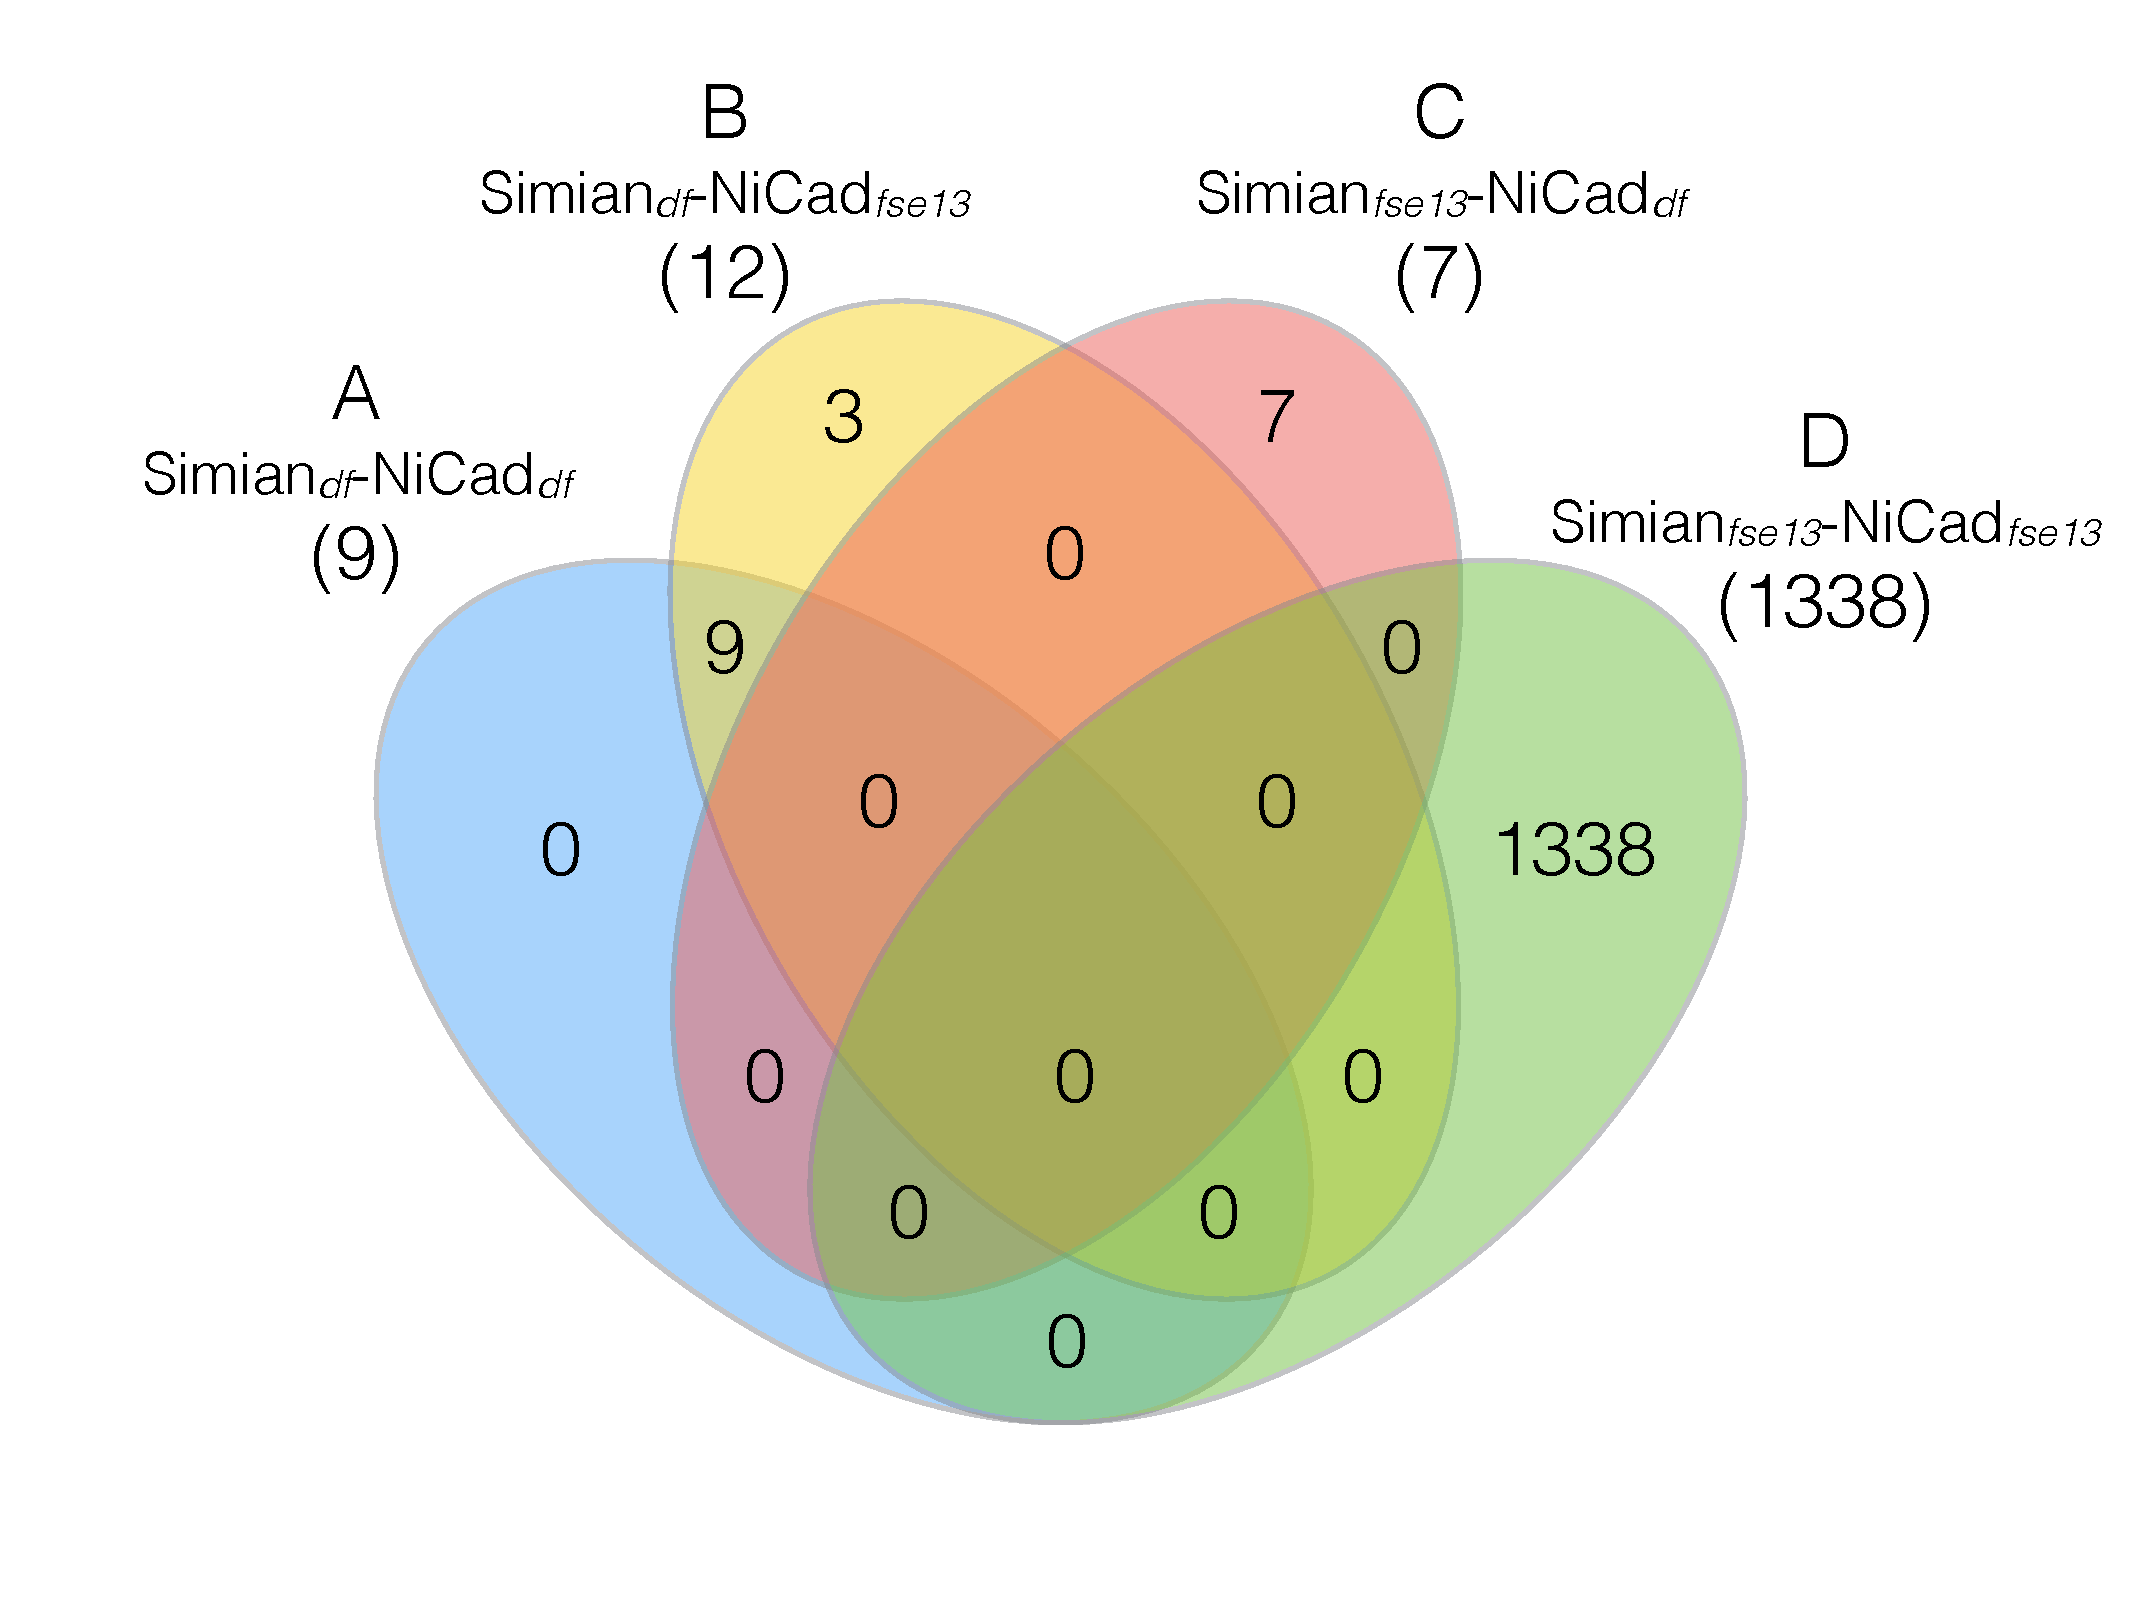
\includegraphics[width=0.9\linewidth]{venn4_pairs_good}
		\caption{\textit{good}-match(0.7) pairs}
		\label{fig:venn4_orig_good}
	\end{minipage}%
	\begin{minipage}{.5\textwidth}
		\centering
		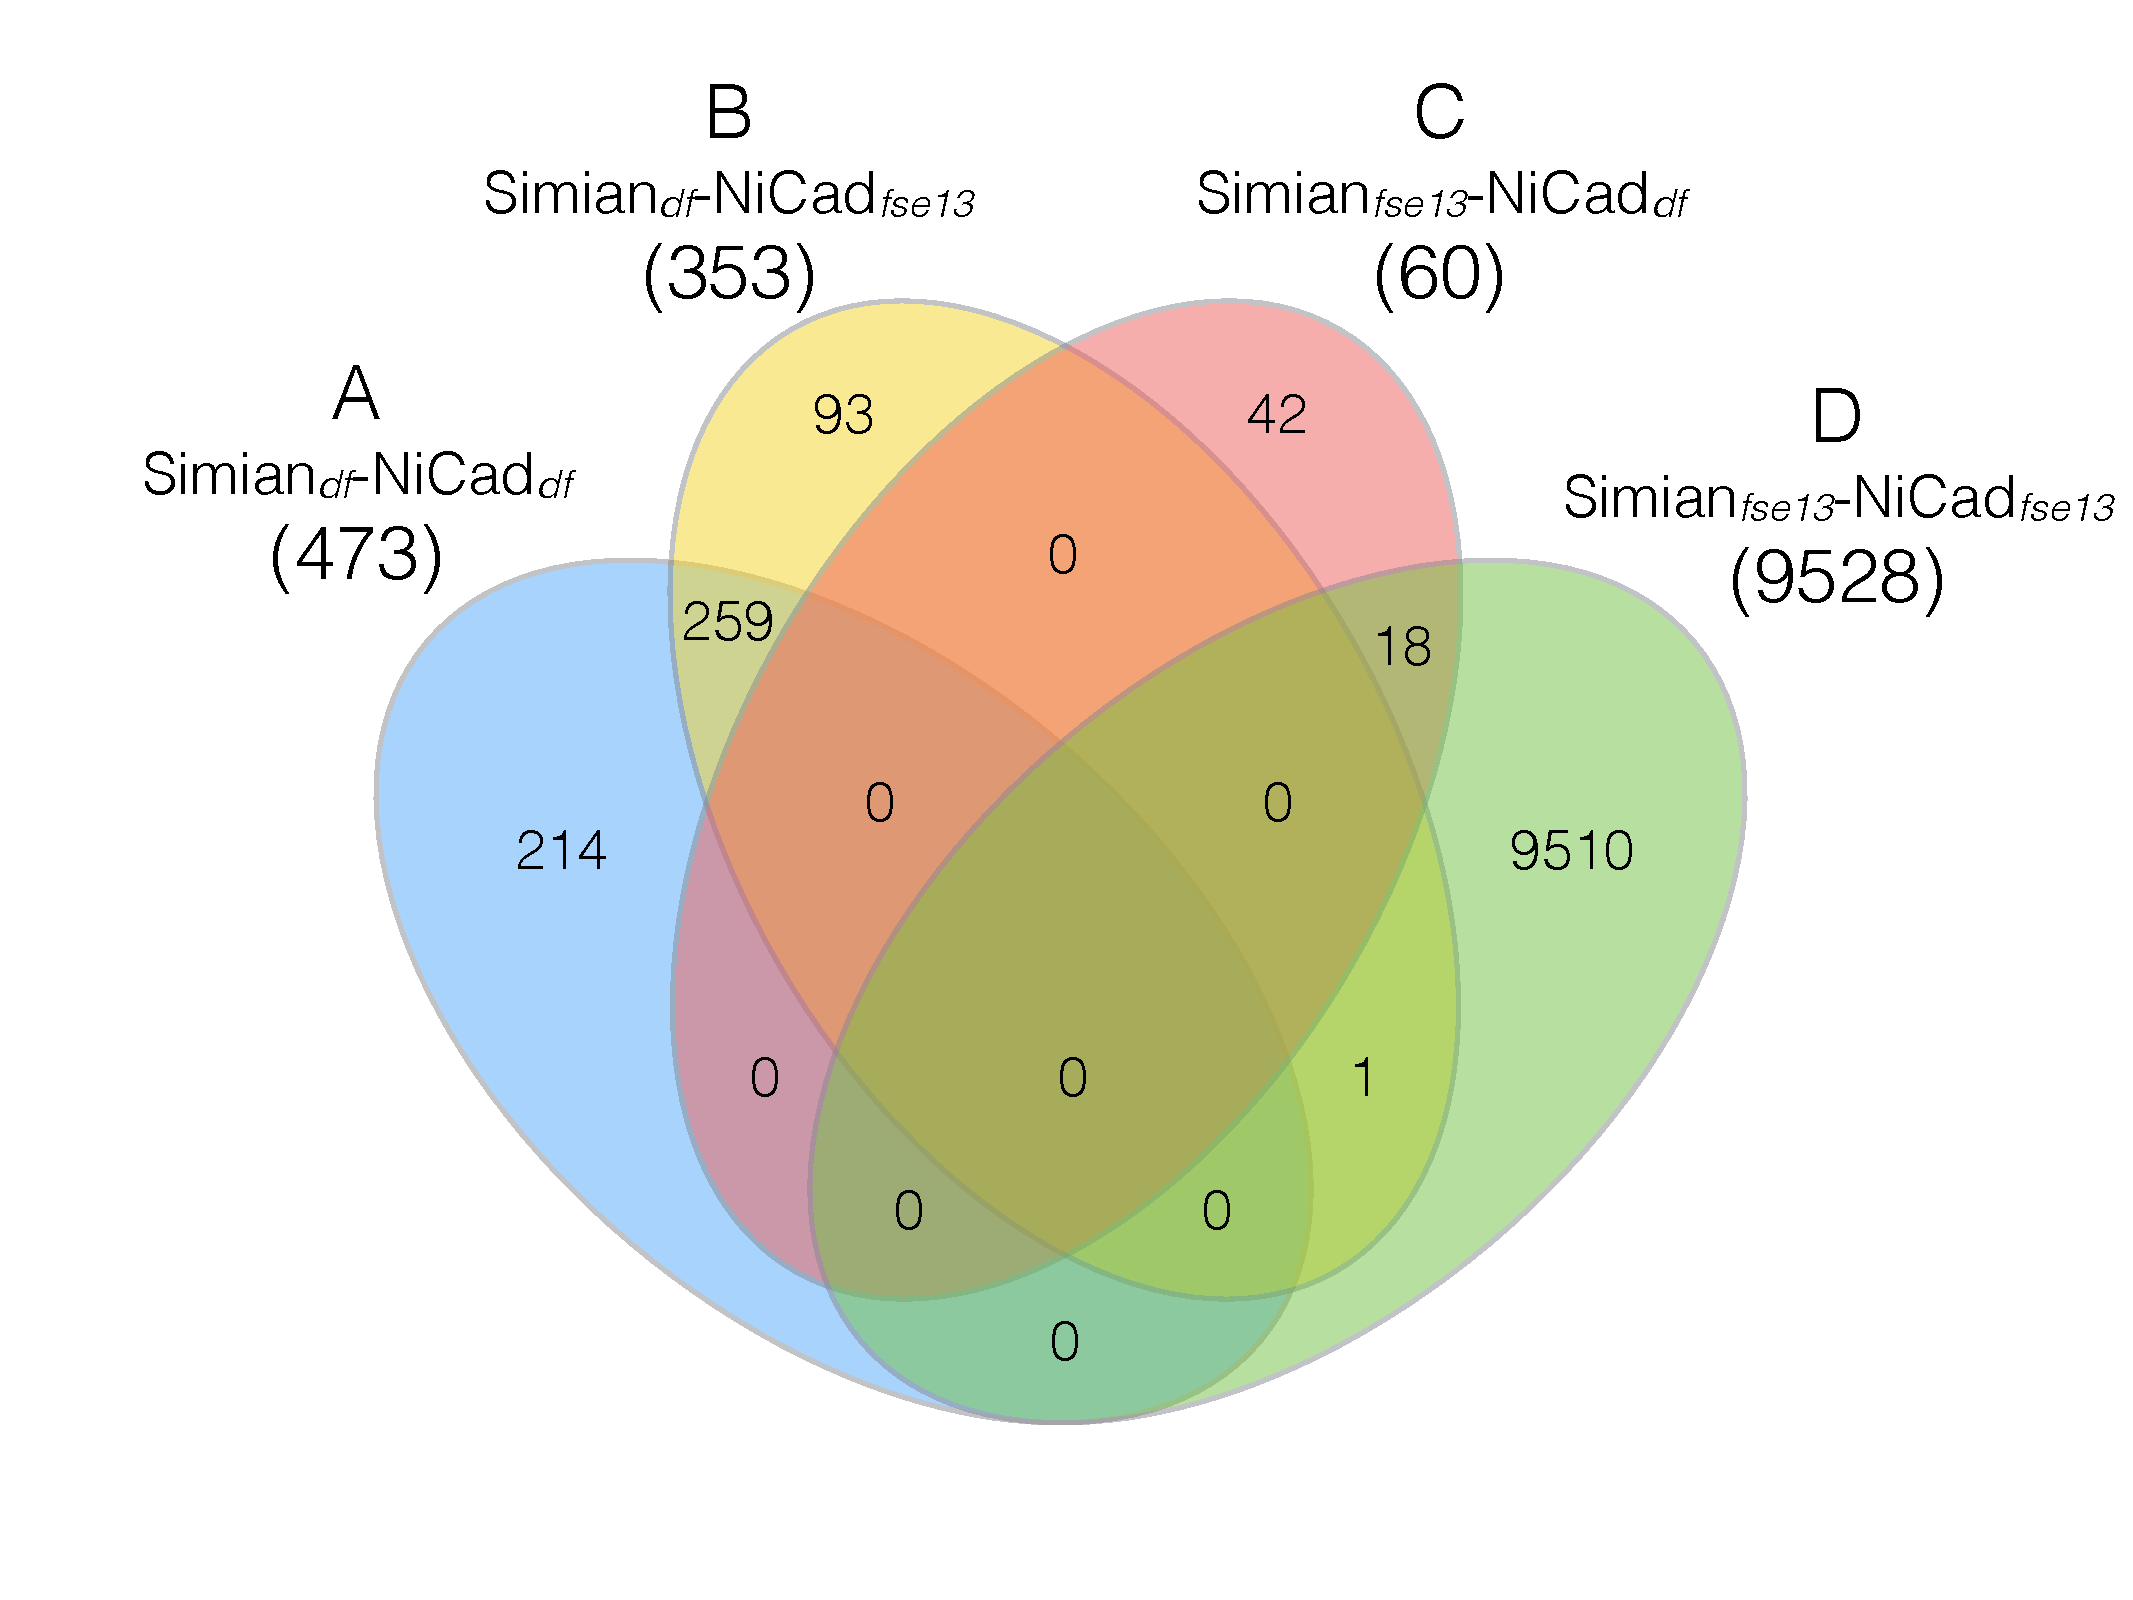
\includegraphics[width=0.9\linewidth]{venn4_pairs_ok}
		\caption{\textit{ok}-match(0.7) pairs}
		\label{fig:venn4_orig_ok}
	\end{minipage}
\end{figure*}

\subsection{Manual investigation of agreement-based clone pairs}
%\subsubsection*{\textbf{Qualitas-\textit{O} (v. 2013-09-01r)}}

%\subsection{Investigation of agreed \textit{good} and \textit{ok}-match clone pairs}

\begin{table*}
	\centering
	\caption{Classifications of clone creation}
	\label{tab:classification_scheme}
	\begin{tabular}{|c|p{13cm}|}
		\hline 
		Category & Descriptions \\ 
		\hline 
		A & Code in Stackoverflow is copied from Qualitas (Q $\rightarrow$ S). \\ 
		\hline 
		A' & Code in Qualitas is copied from Stackoverflow (S $\rightarrow$ Q). \\ 
		\hline 
		B & Code is copied either from each other or a third source (unknown) (S $\leftrightarrow$ Q $\vee$ (T $\rightarrow$ S $\wedge$ T $\rightarrow$ Q)).
		\\ 
		\hline 
		C & Code in both places are copied from a third source T (known) (T $\rightarrow$ S $\wedge$ T $\rightarrow$ Q).
		\\ 
		\hline 
		D & Code is a boiler-plate or IDE auto-generated.
		\\ 
		\hline 
		E & Code in both places initialise a similar/the same object; extend the same class/its subclass; implement the same interface.
		\\ 
		\hline 
		F & Accidental similarity, false clone \\ 
		\hline 
	\end{tabular} 
\end{table*}

The classification scheme is described in Table \ref{tab:classification_scheme} and the classification results are shown in Table \ref{tab:classification_good_o}. We have manually investigated all of the 1,357 \textit{good-match} ones reported by agreement of four different Simian and NiCad settings.  However, for the \textit{ok-match}, we could not investigate all of the 10,139 pairs manually.  According to the distribution of category from \textit{good-match} results, we can see that Simian$_{\textrm{\textit{EvaClone}}}$--NiCad$_{\textrm{\textit{EvaClone}}}$ produces a large number, 1,338, of false positive results (D, E, and F). Thus, we decided to leave them out of the manual investigation of \textit{ok-match} pairs. There are totally 608 \textit{ok-match} pairs that were investigated. The 39 true positive pairs found are combinations of 8 unique Stackoverflow fragments, and 9 unique Qualitas Java files from 6 different projects.

Since we are not certain about the direction of copying in the B-classified pairs, we checked the modification time of each Java file in Qualitas project and compare it to the timestamp of Stackoverflow answers. We found that all Stackoverflow code fragments were posted after their respectively similar Java files in Qualitas project. This means that the copying can only be either (1) Q $\rightarrow$ S or (2) from a third source to both S and Q independently.

%\textbf{Qualitas-\textbf{N}:} We decided to filter out the agreed clone pairs reported by agreement of Simian$_{\mathrm{\textit{EvaClone}}}$-NiCad$_{\mathrm{\textit{EvaClone}}}$ altogether due to its large number of false positive. With the remaining 3 agreements, we did manual investigation of agreed \textit{ok}-match clone pairs from agreements of Simian$_{df}$-NiCad$_{df}$, Simian$_{df}$-NiCad$_{\mathrm{\textit{EvaClone}}}$, and Simian$_{\mathrm{\textit{EvaClone}}}$-NiCad$_{df}$. We had not done any investigation of \textit{good}-match since there were no \textit{good}-match pairs for these 3 agreements. The number of pairs that have been looked at is 6,706 (excluding duplicates). The results are shown in Table.

\begin{table*}
	\centering
	\caption{Qualitas-\textit{O}: Classification results of \textit{good-} and \textit{ok}-match pairs which excludes the subsumed \textit{good}-match and Simian$_{\mathrm{\textit{EvaClone}}}$-NiCad$_{\mathrm{\textit{EvaClone}}}$ pairs.}
	\label{tab:classification_good_o}
	\small
	\begin{tabular}{|l"r|r|r|r|r|r|r|r"r|r|r|r|r|r|r"r|r|r|r|}
		\hline
		Classificaiton & A & A' & B & C & \textbf{Sum} & S$_{u}$ & Q$_u$ & Q$_{up}$ & D  & E & F & \textbf{Sum} & S$_{u}$ & Q$_u$ & Q$_{up}$ & \textbf{Total}  & S$_{u}$ & Q$_u$ & Q$_{up}$\\ 
		\hline 
		\multirow{1}{*}{\textit{good-match(0.7)}}  & 1 & 0 & 1  & 3 & \textbf{5} & 5 & 4 & 4 & 26  & 6 & 1320 & \textbf{1352} & 56 & 402 & 31 & \textbf{1357} & 61 & 406 & 32 \\
		\multirow{1}{*}{\textit{ok-match(0.7)}}  & 8 & 0 & 23  & 8 & \textbf{39} & 8 & 9 & 6 & 480 & 28 & 61 & \textbf{569} & 76 & 60 & 16 & \textbf{608} & 83 & 68 & 19 \\
		\hline
	\end{tabular} 
\end{table*}

%\begin{table}
%	\centering
%	\caption{Classification results of \textit{good-} and \textit{ok}-matches (excluding the subsumed \textit{good}-match pairs).}
%	\label{tab:classification}
%	\begin{tabular}{|l|R{3mm}|R{3mm}|R{3mm}|R{3mm}|R{5mm}|R{3mm}|R{7mm}|R{7mm}|R{3mm}|R{3mm}|R{3mm}|R{3mm}|R{7mm}|R{3mm}|R{7mm}|R{7mm}|}
%		\hline
%		\multirow{2}{*}{Classification}	& \multicolumn{8}{c|}{Qualitas-\textit{O}} & \multicolumn{8}{c|}{Qualitas-\textit{N}} \\ 	\cline{2-17}
%		 & A & A' & B & C & D & E & F & Total 
%		 & A & A' & B & C & D & E & F & Total \\ 
%		\hline 
%		\multirow{1}{*}{\textit{good-match(0.7)}} 
%		& 1 & 0 & 1  & 3 & 26  & 6 & 1,369 & 1,406 
%		& -- & -- & -- & -- & -- & -- & -- & --  \\ \cline{2-8}
%		\hline
%		\multirow{1}{*}{\textit{ok-match(0.7)}} 
%		& 8  & 0 & 36 & 8 & 474 & 57 & 81 & 664 
%		& 2 & 0 & 0 & 0 & 6,676 & 1 & 27 & 6,706 \\ \cline{2-8}
%		\hline
%		TP/FP
%		& \multicolumn{4}{c|}{57} & \multicolumn{3}{c|}{2,013} & 2,070
%		& \multicolumn{4}{c|}{2} & \multicolumn{3}{c|}{6,704} & 6,706 \\ 
%		\hline
%		Unique SO fragments & \multicolumn{4}{c|}{10} & & & & & \multicolumn{4}{c|}{1} & & & & \\
%		\hline
%		Unique Q files & \multicolumn{4}{c|}{13} & & & & & \multicolumn{4}{c|}{1} & & & & \\
%		\hline
%		Unique Q projects & \multicolumn{4}{c|}{8} & & & & & \multicolumn{4}{c|}{1} & & & & \\
%		\hline
%	\end{tabular} 
%\end{table}

\begin{table*}
	\centering
	\caption{Qualitas-\textit{O}: Distribution of classification category A--F according to \textit{good}-match pairs}
	\label{tab:good_classification}
	\small
	\begin{tabular}{|l|r|r|r|r|r|r|r|r|}
		\hline 
		Category   & A   & 	A'   & 	B   & C   & D   &	E   &	F   & Total  \\
		\hline
		Simian$_{df}$--NiCad$_{df}$   & 1 & 0 & 1 & 3 & 0 & 4 & 0 & 9 \\
		Simian$_{df}$--NiCad$_{\textrm{\textit{EvaClone}}}$   & 1 & 0 & 1 & 3 & 1 & 5 & 1 & 12 \\
		Simian$_{\textrm{\textit{EvaClone}}}$--NiCad$_{df}$   & 0 & 0 & 0 & 0 & 7 & 0 & 0 & 7 \\
		Simian$_{\textrm{\textit{EvaClone}}}$--NiCad$_{\textrm{\textit{EvaClone}}}$   & 0 & 0 & 0 & 0 & 18 & 1 & 1,319 & 1,338 \\
		\hline
		Total   &   2   &   0   &  2   &  6   &   26   &   10   & 1,320  & 1,366 \\
		Total (unique)  &   1   &   0   &  1   &  3   &   26   &   6   & 1,320  & 1,352 \\
		\hline
	\end{tabular} 
\end{table*}

\begin{table*}
	\centering
	\caption{Qualitas-\textit{O}: Distribution of classification category A--F  according to the \textit{ok}-match pairs}
	\label{tab:ok_classification}
	\small
	\begin{tabular}{|l|r|r|r|r|r|r|r|r|}
		\hline 
		Category   																										& A   	& 	A' 	& 	B  & C	   & D   	&	E   &	F   & Total  \\
		\hline
		Simian$_{df}$--NiCad$_{df}$        & 3 	& 0 	& 10	& 6 	& 433  & 5	& 7  &  464 \\
		Simian$_{df}$--NiCad$_{\textrm{\textit{EvaClone}}}$   									& 8 	& 0 	& 22	& 4	& 250 & 25  & 32 &  341 \\
		Simian$_{\textrm{\textit{EvaClone}}}$--NiCad$_{df}$   									& 0 	& 0 	& 0 	& 0 	 & 29 	  & 0 		& 24 	& 53 \\
		\hline
		Total   &   11  &   0   &  32   &  10   &   712   &   30   & 63  & 858 \\
		Total (unique)  &   8  &   0   &  23   &  8   &  480  &  28  & 61  & 608 \\
		\hline
	\end{tabular} 
\end{table*}

%\subsubsection{Qualitas-\textit{N} (v. 2016-08-05)}
%We decided to filter out the agreed clone pairs reported by agreement of Simian$_{\mathrm{\textit{EvaClone}}}$-NiCad$_{\mathrm{\textit{EvaClone}}}$ altogether due to its large number of false positive. With the remaining 3 agreements, we did manual investigation of agreed \textit{ok}-match clone pairs from agreements of Simian$_{df}$-NiCad$_{df}$, Simian$_{df}$-NiCad$_{\mathrm{\textit{EvaClone}}}$, and Simian$_{\mathrm{\textit{EvaClone}}}$-NiCad$_{df}$. We had not done any investigation of \textit{good}-match since there were no \textit{good}-match pairs for these 3 agreements. The number of pairs that have been looked at is 6,706 (excluding duplicates). The results are shown in Table \ref{tab:classification_good_n}.
%
%\begin{table}
%	\centering
%	\caption{Qualitas-\textit{N}: Classification results of \textit{good-} and \textit{ok}-matches (excluding the subsumed \textit{good}-match pairs).}
%	\label{tab:classification_good_n}
%	\begin{tabular}{|l"r|r|r|r|r|r|r|r"r|r|r|r|r|r|r"r|r|r|r|}
%		\hline
%		Classificaiton & A & A' & B & C & Sum & S$_{u}$ & Q$_u$ & Q$_{up}$ & D  & E & F & Sum & S$_{u}$ & Q$_u$ & Q$_{up}$ & Total  & S$_{u}$ & Q$_u$ & Q$_{up}$\\ 
%		\hline 
%		\multirow{1}{*}{\textit{good-match(0.7)}}  & - & - & - & - & - & - & - & - & - & - & - & - & - & - & - & - & - & - & - \\
%		\multirow{1}{*}{\textit{ok-match(0.7)}}  & 2 & 0 & 0 & 0 & & & & & 6676 & 1 & 27 & & & & & 6706 & & & \\
%		\hline
%	\end{tabular} 
%\end{table}

%\begin{table}
%	\centering
%	\caption{Classification results of 6,706 \textit{ok}-matches of Simian$_{df}$-NiCad$_{df}$, Simian$_{df}$-NiCad$_{\mathrm{\textit{EvaClone}}}$.}
%	\label{tab:classification_new}
%	\begin{tabular}{|l|r|r|r|r|r|r|r|r|}
%		\hline 
%		Classification & A & A' & B & C & D & E & F & Total \\ 
%		\hline
%		\multirow{1}{*}{\textit{good-match(0.7)}} & -- & -- & -- & -- & -- & -- & -- & -- \\ \cline{2-8}
%		\hline
%		\multirow{1}{*}{\textit{ok-match(0.7)}}  \\ \cline{2-8}
%		\hline
%		\multirow{3}{*}{TP/FP} & \multicolumn{4}{c|}{2} & \multicolumn{3}{c|}{\multirow{3}{*}{6704}} & \multirow{3}{*}{6706} \\ 
%		& \multicolumn{4}{l|}{\textit{1 unique SO fragments}} & \multicolumn{3}{c|}{} & \\
%		& \multicolumn{4}{l|}{\textit{1 unique Q files}} & \multicolumn{3}{c|}{} & \\
%		\hline
%	\end{tabular} 
%\end{table}

%\begin{table}
%	\centering
%	\caption{Qualitas-\textit{N}: Distribution of classification category A--F  according to the \textit{ok}-match pairs}
%	\label{tab:ok_classification_new}
%	\begin{tabular}{|l|r|r|r|r|r|r|r|r|}
%		\hline 
%		Category   																										& A   	& 	A' 	& 	B  & C	   & D   	&	E   &	F   & Total  \\
%		\hline
%		Simian$_{df}$--NiCad$_{df}$ & 0 & 0	& 0 & 0 & 6603 & 1 & 0 & 6604 \\
%		Simian$_{df}$--NiCad$_{\textrm{\textit{EvaClone}}}$ 
%		& 2 	& 0 	& 0 	& 0 	& 73 	 & 0 	  & 4 		&  79 \\
%		Simian$_{\textrm{\textit{EvaClone}}}$--NiCad$_{df}$   									
%		& 0 	& 0 	& 0 	& 0 	 & 0 	  & 0 		& 23 	& 23 \\
%		\hline
%		Total   & 2  	&   0   & 0   	&  0   &   6676   &   1   & 27  & 6706 \\
%		\hline
%	\end{tabular} 
%\end{table}

\begin{figure*}
	\centering
	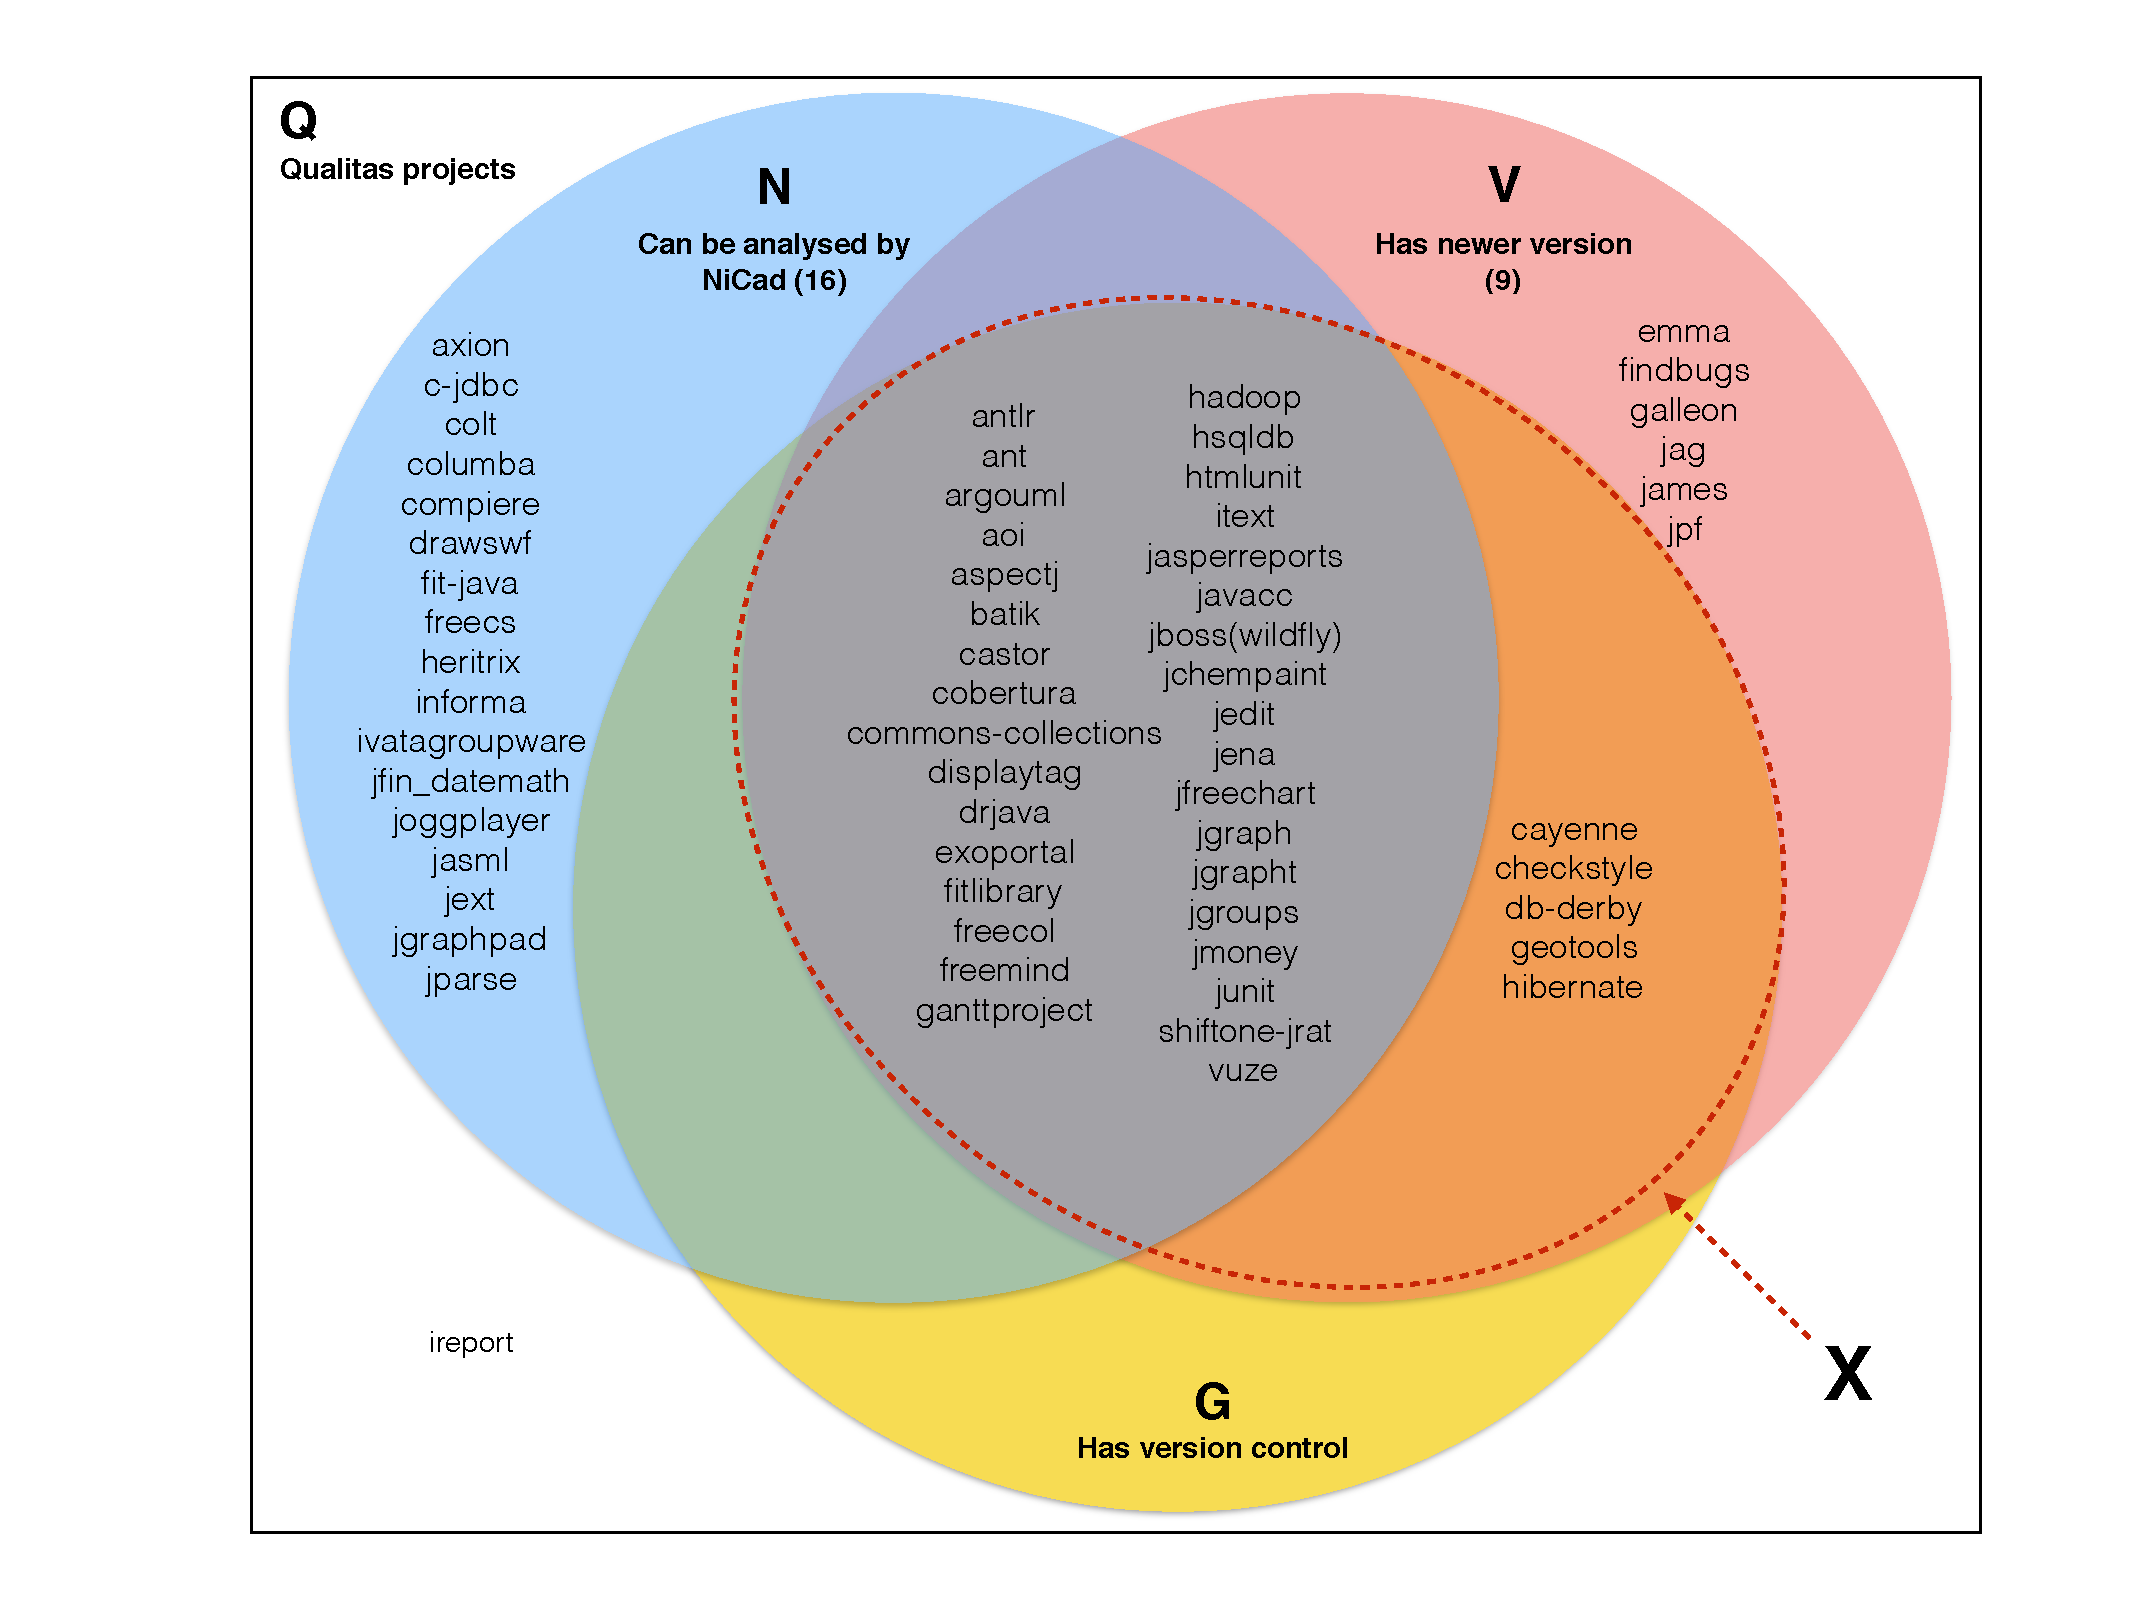
\includegraphics[width=0.7\linewidth]{n+v+g}
	\caption{Qualitas projects categorised by NiCad's results, existence of newer versions, and version control}
	\label{fig:n+v+g}
\end{figure*}

\subsection{Non-agreement based clone pairs}
In the preliminary stage of our experiment, we found that there are 41 Stackoverflow fragments reported by Simian with default configurations. However, only 10 of them appear in the new results using tool's agreement. Thus, we further investigated the clone pairs reported by Simian and NiCad but \textit{without} an agreement. 

With our 4 settings, we decided to investigate only 2 settings, Simian$_{df}$, and NiCad$_{df}$, and drop Simian$_{\mathrm{\textit{EvaClone}}}$ and NiCad$_{\mathrm{\textit{EvaClone}}}$ due to their large number of false positives as shown in Table \ref{tab:good_classification} and \ref{tab:ok_classification}. With the 2 selected settings, we investigated clone pairs having the minimum clone size of 10 SLOC as they are meaningful and tend to be real clone in modern clone detection \cite{Sajnani2016}. 

For Simian$_{df}$, there were 9,383 clone pairs reported by the tool. Out of 9,383 pairs, 140 of them are the ones found in \textit{ok-}pairs using agreement-based detection. We filtered the results further by removing false positives such as similar equals(), hashCode() methods, getters and setters out by using regular expression. We managed to remove 8,956 pairs using this method. Eventually, there were 287 clone pairs remaining for manual investigation. For NiCad$_{df}$, we obtained 7,040 clone pairs to look at which is infeasible for manual investigation. Hence, result filtering was also needed. However, regular expressions could not be used effectively as in Simian's case since NiCad allowed clones that are different at keywords/variable names or even added/deleted lines. So we decided to filter the results by selecting pairs that pass stricter clone criteria with $\mathrm{UPI} = 0.2$. By reducing the UPI to 0.2, there were totally 166 pairs left. Out of 166, 52 are \textit{ok}-pairs and 114 are remaining pairs for manual check (18 pairs are from \textit{cayenne} and \textit{iReport} that could not be analysed using UPI = 0.3). The statistics of the clones and classification results are reported in Table \ref{tab:classification_indv_stats} and \ref{tab:classification_indv}.

%We selected only Stackoverflow fragment and Qualitas files that have never been looked at before in the previous investigation. If many clone pairs having the same Stackoverflow fragment and Qualitas file, we keep only the largest one. The reason for having this criteria is that we found a lot of duplicate clone pairs with the same classifications from either Stackoverflow fragments or Qualitas files. The classification results are shown in Table \ref{tab:classification_indv}. 

\begin{table*}
	\centering
	\caption{Statistics of Simian$_{df}$ and NiCad$_{df}$ clone pairs.}
	\label{tab:classification_indv_stats}
	\small
	\begin{tabular}{l|r|r|r|r}
		\hline 
		Tool & Clone pairs & \textit{ok}-pairs & filtered pairs & remaining pairs \\ 
		\hline 
		\multirow{1}{*}{\textit{Simian$_{df}$}} & 9383 & 140 & 8956 & 287 \\
		\hline
		\multirow{1}{*}{\textit{NiCad$_{df}$}} & 7040  & 226 & 6700 & 114 \\
		\hline
	\end{tabular} 
\end{table*}

\subsection{Manual investigation of non-agreement based clone pairs}
%\subsubsection*{\textbf{Qualitas-\textit{O} (v. 2013-09-01r)}}
We performed manual investigation of the clone pairs reported by Simian$_{df}$ and NiCad$_{df}$ in the same way as the agreement-based clone pairs. The results of the manual investigation is reported in Table \ref{tab:classification_indv}.

\begin{table*}
	\centering
	\caption{Classification results of 292 Simian$_{df}$ and 114 NiCad$_{df}$ individual unique pairs.}
	\label{tab:classification_indv}
	\small
	\begin{tabular}{|l|r|r|r|r|r|r|r|r|r|r|r|r|r|r|r|r|r|r|r|}
		\hline 
		Tool/Classification & A & A' & B & C & \textbf{Sum} & S$_{u}$ & Q$_{u}$ & Q$_{up}$ & D & E & F & \textbf{Sum}  & S$_{u}$ & Q$_{u}$ & Q$_{up}$ & \textbf{Total} & S$_{u}$ & Q$_{u}$  & Q$_{up}$  \\ 
		\hline 
		\multirow{1}{*}{\textit{Simian$_{df}$}} & 35 & 0 & 89 & 7 & \textbf{133} & 68 & 57 & 23 & 13 & 10 & 133 & \textbf{159} & 39 & 69 & 23 & \textbf{287} & 103 & 121 & 31 \\
		\hline
		\multirow{1}{*}{\textit{NiCad$_{df}$}} & 4  & 0 & 5 & 0 & \textbf{9} & 9 & 5 & 4 & 24 & 3 & 78 & \textbf{105} & 41 & 39 & 12 & \textbf{114} & 48 & 44 & 14 \\ 
		\hline
		%		\multirow{1}{*}{\textit{NiCad$_{df}$}*} & 4  & 0 & 1 & 0 & \textbf{5} & 4 & 5 & 3 & 23 & 1 & 67 & \textbf{91} & 28 & 31 & 10 & \textbf{96} & 33 & 37 & 13 \\ 
		%		\hline
	\end{tabular} 
\end{table*}

%\subsection{Summary of true online clone pairs}
\begin{table}[H]
	\centering
	\caption{Numbers of true online clone pairs (A+A'+B+C) found by manual investigation}
	\label{tab:classification_true_pairs_summary}
	\begin{tabular}{l|r|r|r|r|r}
		\hline 
		Tool & A & A' & B & C & Total \\
		\hline
		\textit{good}-pairs & 1 & 0 & 1 & 3 & 5 \\
		\textit{ok}-pairs & 8 & 0 & 23 & 8 & 39 \\
		Simian$_{df}$ pairs & 35 & 0 & 89 & 7 & 131 \\
		NiCad$_{df}$ pairs & 4 & 0 & 5 & 0 & 9 \\
		\hline 
		Total & 48 & 0 & 118 & 18 & 184 \\
		\hline
	\end{tabular} 
\end{table}

\begin{figure*}
	\centering
	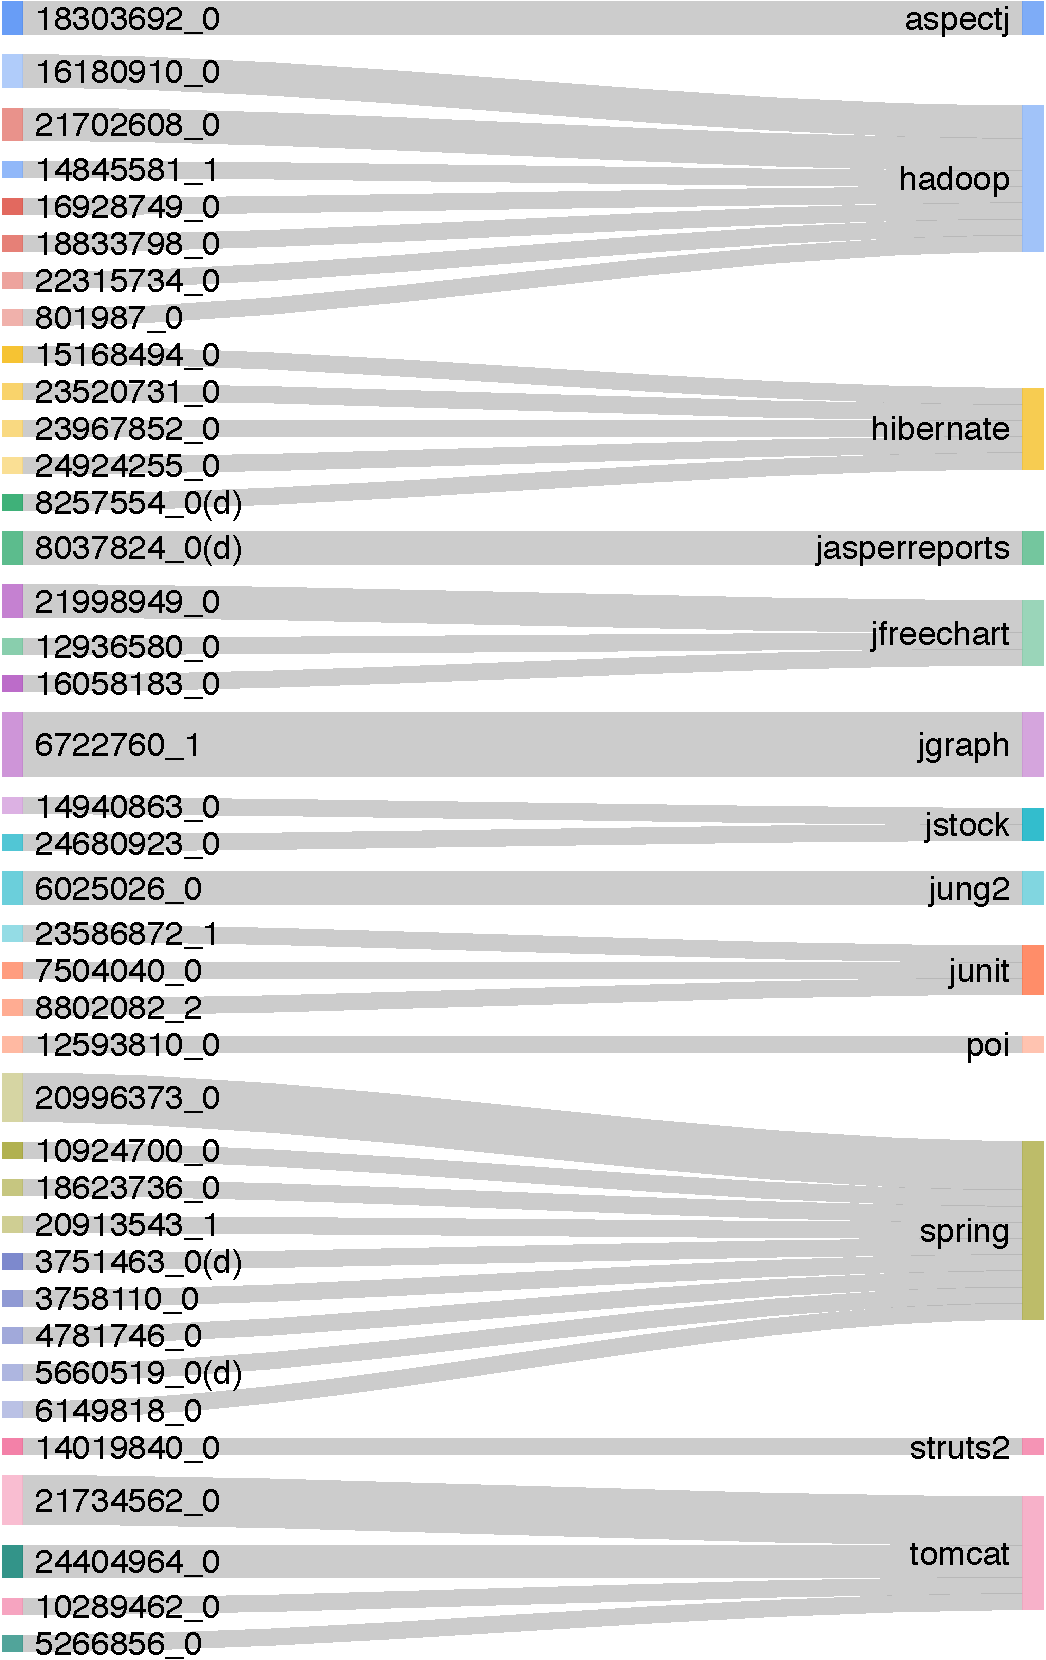
\includegraphics[width=1\linewidth]{Sankey_proj}
	\caption{Relationships between 184 true online code clone found between Stackoverflow and Qualitas projects}
	\label{fig:sankey}
\end{figure*}

%\subsubsection{Qualitas-\textit{N} (v. 2016-08-05)}

\section{Effects of online code clone}

In this study, we are interested in the effects of online code clones to software development. From the manual investigation of 184 true online clone pairs, we found that there are two potential issues: stale online code, and software licensing violation.

\subsection{Issue~1:~stale online code}
Stale online code occurs when a piece of code has been copied from a software project to Stackoverflow, and later it has been changed in the original project. However, in this situation, the copy is still unchanged. Since the code were updated due to various possible reasons including bug fixing, this can cause a problem if developers reuse stale online code from Q\&A websites such as Stackoverflow. They might also introduce the same unfixed bug(s) into the software. To discover stale online code, we focus on the true online clone pairs that are copied in the direction of Q $\rightarrow$ S (class-\textit{A} online clone pairs) in Table \ref{tab:classification_true_pairs_summary} which results in 48 pairs selected. We restricted it further to only the ones having versioning system so we can trace changes made to these clone pairs. Fortunately, all of the pairs were from projects with either git or svn so we did not remove any pair from this set. 

%Our intuition behind his issue comes from a situation where a piece of code has been copied from a Qualitas project and posted on Stackoverflow. Later, that piece of code has been modified further to accommodate changes in the projects (or any other reasons). However, even the code in Qualitas project is already updated, the one posted on Stackoverflow is not changed. This results in outdated online code which can cause problems when programmers copy and use it in their projects.

%We decided to ignore NiCad results from this analysis due to its failure of clone clustering and renaming on some projects.  Thus, the 39 projects are the ones that can be analysed by Simian, have newer versions than the versions in Qualitas-\textit{O}, and have code version control system (either git or svn). %After filtering, there are 141 pairs removed because 45 of them do not have new versions (7 from c-jdbc, 21 from Compiere, 7 from heritrix, and 10 from iReport) and 4 of them we could not find source code with version control (2 from findbugs, 1 from jag, and 1 from jgraphpad). Finally there were 134  pairs remaining. %We are interested in clone pairs that were changed after they appeared on Stackoverflow.

The manual investigation of 48 class-A online clone pairs reveals that there are 30 stale clones. They are clone pairs that were copied from Qualitas projects to Stackoverflow and marked as \textit{accepted} answers.  The investigation results are described in Table \ref{tab:stale_code}.

\begin{table}[H]
	\centering
	\caption{Investigation of stale code clones from the online clone pairs}
	\label{tab:stale_code}
	\begin{tabular}{l|r|r|r}
		\hline 
		Project & Pairs & Stale & Fresh \\
		\hline
		apache-ant & 1 & 0 & 1 \\
		aspectj & 2 & 2 & 0 \\
		hadoop & 14 & 9 & 5 \\
		hibernate & 16 & 5 & 11 \\
		jasperreports & 2 & 2 & 0 \\
		jfreechart & 4 & 4 & 0 \\
		jgraph & 5 & 5 & 0 \\
		jgrapht & 1 & 0 & 1 \\
		junit & 3 & 3 & 0 \\
		\hline
		Total & 48 & 30 & 18 \\
		\hline
	\end{tabular} 
\end{table}

\begin{table*}
	\centering
	\caption{30 stale code clones found by a manual investigation}
	\label{tab:stale_code_details}
	\begin{tabular}{r|l|r|r}
		\hline 
		No. & File & Stackoverflow Q\&A & Change date \\
		\hline
		1 & aspectjtools1.6.9-src/../Agent.java & 18303692 & 2015-09-08 \\
		2 & aspectjweaver1.6.9-src/../Agent.java & 18303692 & 2015-09-08 \\
		3 & hadoop-1.0.0/../WritableComparator.java & 22315734 & 2014-11-20 \\
		4 & hadoop-1.0.0/../StringUtils.java & 801987 & 2013-02-04 \\
		5 & hadoop-1.0.0/../DBCountPageView.java & 21702608 & 2011-06-12 \\
		6 & hadoop-1.0.0/../DBCountPageView.java & 21702608 & 2011-06-12 \\
		7 & hadoop-1.0.0/../LineRecordReader.java & 16180910 & 2011-07-25 \\
		8 & hadoop-1.0.0/../LineRecordReader.java & 16180910 & 2011-07-25 \\
		9 & hadoop-1.0.0/../JobSubmissionFiles.java & 14845581 & 2012-06-25 \\
		10 & hadoop-1.0.0/../TextOutputFormat.java & 16928749 & 2011-06-12 \\
		11 & hadoop-1.0.0/../TestJobCounters.java & 18833798 & 2011-06-12 \\
		12 & hibernate-release-4.2.2.Final/../SettingsFactory.java & 8257554 & 2011-03-11 (deleted) \\
		13 & hibernate-release-4.2.2.Final/../Example.java & 24924255 & 2013-04-23 \\
		14 & hibernate-release-4.2.2.Final/../SQLServer2005LimitHandler.java.java & 23967852 & 2013-04-23 \\
		15 & hibernate-release-4.2.2.Final/../ConnectionProviderInitiator.java & 15168494 & 2016-02-24 \\
		16 & hibernate-release-4.2.2.Final/../SchemaUpdate.java & 23520731 & 2016-02-05 \\
		17 & jasperreports-3.7.4/../JRVerifier.java & 8037824 & 2011-05-20 (deleted) \\
		18 & jasperreports-3.7.4/../JRVerifier.java & 8037824 & 2013-12-08 \\
		19 & jasperreports-3.7.4/../SpiderWebPlot.java & 21998949 & 2013-11-22 \\
		20 & jasperreports-3.7.4/../SpiderWebPlot.java & 21998949 & 2013-11-22 \\
		21 & jasperreports-3.7.4/../AbstractXYItemRenderer.java & 12936580 & 2016-01-16 \\
		22 & jfreechart-1.0.13/../KeyToGroupMap.java & 16058183 & 2013-07-03 \\
		23 & jgraph-latest-bsd-src/../GroupingRemoving.java & 6722760 & 2005-xx-xx (rewritten) \\
		24 & jgraph-latest-bsd-src/../HelloWorld.java & 6722760 & 2005-xx-xx (rewritten) \\
		25 & jgraph-latest-bsd-src/../HelloWorld.java & 6722760 & 2005-xx-xx (rewritten) \\
		26 & jgraph-latest-bsd-src/../HelloWorld.java & 6722760 & 2005-xx-xx (rewritten) \\
		27 & jgraph-latest-bsd-src/../HelloWorld.java & 6722760 & 2005-xx-xx (rewritten) \\
		28 & junit-4/org/junit/Assert.java & 23586872 & 2015-05-12 \\
		29 & junit-4/../ExpectException.java & 8802082 & 2014-05-26 \\
		30 & junit-4/../ExternalResource.java & 7504040 & 2016-06-25 \\
		\hline
	\end{tabular} 
\end{table*}

\subsection{Issue~2:~software licensing violation}
Software licensing is vital in software industry. Violation of software license can have a major impact to the delivery of the software and also lead to legal issues. It is an emerging area that software engineering research community is paying attention to. For example, there are studies of automatic technique to identify software licensing from source code files \cite{German2010} and the evolution of licenses in open source projects \cite{DiPenta2010}.

In our study, we tackle another possible situation of software licensing issue caused by code cloning to Q\&A websites. We found that there are at least 48 pieces of code have been copied from 9 open source projects to Stackoverflow as examples. These 9 open source projects come with software licenses. However, the licensing information are mostly missing from these clones. If developers copy and reuse these pieces of code in their projects, a licensing conflict can quietly happen without realisation of the developers. 

\section{Investigation of Missing A/B Clone Pairs Reported by Simian$_{df}$}
We investigated the 41 clone pairs previously reported by Simian with default configurations and manually investigated. The 41 pairs were searched for in 4 new results sets: Simian$_{df}$, Simian$_{\mathrm{\textit{EvaClone}}}$, NiCad$_{df}$, NiCad$_{\mathrm{\textit{EvaClone}}}$. The investigation results are shown in Table \ref{tab:search}.

\begin{table}
	\centering
	\caption{Results of matching the original 41 Simian(default) pairs in the pretty-printed result sets}
	\label{tab:search}
	\begin{tabular}{l|r|r}
		\hline 
		Settings & Found & Not found \\ 
		\hline 
		Simian$_{df}$  &  40 & 1* \\ 
		\hline 
		Simian$_{\mathrm{\textit{EvaClone}}}$ & 0 & 41  \\ 
		\hline 
		NiCad$_{df}$  & 17 & 24 \\ 
		\hline 
		NiCad$_{\mathrm{\textit{EvaClone}}}$ &  24 & 17 \\ 
		\hline 
	\end{tabular} 
\end{table}

The single missing Stackoverflow fragment (19051537\_0.java) (denoted by *) is one of the 11 false clones generated by Simian. It is removed from the results of the pretty-printed version because it is an outlier. The rest are missing because of different parameter settings.

\section{Simian's Parameters}

We have carefully investigated the effects of the Simian's parameter \texttt{-balanceSquareBrackets+}. I found that it works in the expected way of handling a pair of brackets (\texttt{[},\texttt{]}) that span over multiple lines. For example, the two code fragments in Figure \ref{fig:two_frags} would match by having \texttt{-balanceSquareBrackets+} enabled. However, the \texttt{-balanceSquareBrackets+} parameter only works on a small testing environment having toy programs or only small pairs from the full datasets. It does not work with the full complete set of 144,075 Stackoverflow fragments and Qualitas projects. Please find the summary of all the testing scenarios in Table \ref{tab:summary}. %I found that this pair is missing if I turned on \texttt{-balanceSquareBrackets+}.

\noindent\begin{figure*}
	\scriptsize
	\begin{lstlisting}[frame=single,style=base]
	1   public class MagicSquare {                           public class MagicSquare2 {
	2       private int[][] square;                              @private int[@
	3       private boolean[] possible;                                      @][@
	4       private int totalSqs;                                            @] square;@
	5       private int sum;                                     private boolean[] possible;
	6       private int numsquares;                              private int totalSqs;
	7       public static void main ( String[] args ) {          private int sum;
	8       MagicSquare m = new MagicSquare ( 3 );               private int numsquares;
	9                                                            public static void main ( String[] args ) {
	10                                                           MagicSquare m = new MagicSquare ( 3 );
	\end{lstlisting}
	\caption{Two identical fragments with only differences in locations of the square brackets. All 7 lines are reported by Simian if \small\texttt{-balanceSquareBrackets+} \normalsize is enabled. If not, the clone pairs is reported as \newline (MagicSquare.java [3,8], MagicSquare2.java [5,10]).} 
	\label{fig:two_frags}
\end{figure*}

\begin{table*}
	\caption{Simian's \texttt{-balanceSquareBrackets+} (\texttt{-bsb+}) is observed to have unpredictable behaviours when running against big datasets. $\textrm{\textit{CP}}_2$ means the reported clone(s) do not contain lines having dislocated brackets ($L_b$) (i.e. $\textrm{\textit{CP}}_2 = \textrm{\textit{CP}}_1 - L_b$).}
	\label{tab:summary}
	\centering
	\small\begin{tabular}{l|p{6cm}|c|c|c}
		\hline 
		\multirow{2}{*}{\textbf{Project 1}} & \multirow{2}{*}{\textbf{Project 2}} & \textbf{Dislocated} & \multirow{2}{*}{\textbf{-bsb+}} & \textbf{Clones pair} \\ 
		& & \textbf{brackets?} & & \textbf{reported} \\
		\hline
		\hline
		\multicolumn{5}{l}{\textit{Only run Simian against the pair}} \\
		\hline
		MagicSquare.java & MagicSquare\_exact\_copy.java & no & 0,1 & $\textrm{\textit{CP}}_1$ \\
		MagicSquare.java & MagicSquare2.java & yes & 0 & $\textrm{\textit{CP}}_2$ \\ 
		MagicSquare.java & MagicSquare2.java & yes & 1 & $\textrm{\textit{CP}}_1$ \\
		\hline
		%\hline
		%\multicolumn{5}{c}{\textit{Only run Simian against the pair}} \\
		%\hline
		stackoverflow/4298836\_0.java & Qualitas/aoisrc281/../ExprModule.java & no & 0 & $\textrm{\textit{CP}}_3$ \\ 
		stackoverflow/4298836\_0.java & Qualitas/aoisrc281/../ExprModule.java & no & 1 & $\textrm{\textit{CP}}_3$ \\ 
		stackoverflow/4533682\_1.java & Qualitas/cobertura-1/../TouchCollector.java & no & 0 & $\textrm{\textit{CP}}_4$ \\ 
		stackoverflow/4533682\_1.java & Qualitas/cobertura-1/../TouchCollector.java & no & 1 & $\textrm{\textit{CP}}_4$ \\ 
		\hline 
		\hline
		\multicolumn{5}{l}{\textit{Run Simian against the complete stackoverflow data and the project}} \\
		\hline
		stackoverflow/4298836\_0.java & Qualitas/aoisrc281/../ExprModule.java & no & 0 & $\textrm{\textit{CP}}_3$ \\ 
		\cellcolor{red!10}stackoverflow/4298836\_0.java & \cellcolor{red!10}Qualitas/aoisrc281/../ExprModule.java & \cellcolor{red!10}no & \cellcolor{red!10}1 & \cellcolor{red!10}-- \\ 
		\hline
		stackoverflow/4533682\_1.java & Qualitas/cobertura-1/../TouchCollector.java & no & 0 & $\textrm{\textit{CP}}_4$ \\ 
		\cellcolor{red!10}stackoverflow/4533682\_1.java & \cellcolor{red!10}Qualitas/cobertura-1/../TouchCollector.java & \cellcolor{red!10}no & \cellcolor{red!10}1 & \cellcolor{red!10}-- \\
		\hline 
	\end{tabular} 
\end{table*}

\section{Threats to Validity}

\section{Related Work}
\begin{itemize}
	\item Code clones 
		\begin{itemize}
			\item Definition: Baxter et al. \cite{Baxter1998}
			\item Comparison of clone detectors: \cite{Roy2008, Ragkhitwetsagul2016,Svajlenko2014}
			\item NiCad \cite{Roy2008,Cordy}
			\item Simian \cite{simian}
			\item Clone taxonomy \cite{Kapser2003}
			\item Clone evolution \cite{Pate2013,Mondal2011}
			\item Comparing Quality Metrics for Cloned and non cloned Java Methods : A Large Scale Empirical Study \cite{Saini2016}.
		\end{itemize}
	\item Agreement-based Clone Detection
	\begin{itemize}
		\item Bellon's framework \cite{Bellon2007}.
		\item EvaClone \cite{Wang2013}
		\item Hybrid \cite{Funaro2010}
	\end{itemize}
	\item Software licensing
	\begin{itemize}
		\item Code siblings \cite{German2009}, Ninka -- Automatic indification of SW license \cite{German2010}, Evolution of SW licensing \cite{DiPenta2010}
	\end{itemize}

	\item Stackoverflow
	\begin{itemize}
		\item Code example \cite{Nasehi2012}
		\item Search for code in Stackoverflow \cite{Diamantopoulos2015,Keivanloo2014,Park2014}
	\end{itemize}
\end{itemize}

\section{Conclusions}
This paragraph will end the body of this sample document.
Remember that you might still have Acknowledgments or
Appendices; brief samples of these
follow.  There is still the Bibliography to deal with; and
we will make a disclaimer about that here: with the exception
of the reference to the \LaTeX\ book, the citations in
this paper are to articles which have nothing to
do with the present subject and are used as
examples only.
%\end{document}  % This is where a 'short' article might terminate

%ACKNOWLEDGMENTS are optional
\section{Acknowledgments}
This section is optional; it is a location for you
to acknowledge grants, funding, editing assistance and
what have you.  In the present case, for example, the
authors would like to thank Gerald Murray of ACM for
his help in codifying this \textit{Author's Guide}
and the \textbf{.cls} and \textbf{.tex} files that it describes.

%
% The following two commands are all you need in the
% initial runs of your .tex file to
% produce the bibliography for the citations in your paper.
\bibliographystyle{abbrv}
\bibliography{sigproc}  

\end{document}
